\subsection{UI5 Pantalla principal gerente}

\subsubsection{Objetivo}
    Seleccionar alguna funcionalidad a realizar permitida para el gerente.

\subsubsection{Diseño}
    Esta pantalla aparece al iniciar sesión como Gerente.

\begin{figure}[htbp!]
        \centering
            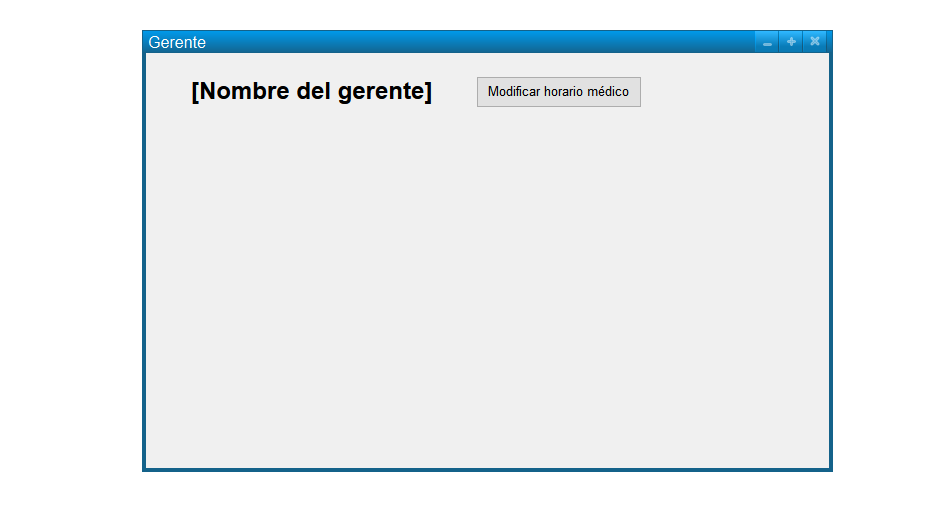
\includegraphics[width=0.8\textwidth]{images/UIGerente1}
        \caption{Pantalla principal de Gerente}
    \end{figure}


\subsubsection{Entradas}
  Ninguna

\subsubsection{Comandos}
\begin{itemize}
    \item \IUbutton{Modificar horario médico}: Permite realizar la transacción descrita en \UCref{CU5}
\end{itemize}

\subsubsection{Mensajes}
   Ninguno.
   
\subsection{UI6 Pantalla modificar horario listado de médicos}

\subsubsection{Objetivo}
   Seleccionar un médico para modificar su horario en el que está disponible para realizar consultas.

\subsubsection{Diseño}
    Esta pantalla aparece al oprimir \IUbutton{Modificar horario médico} de la \IUref{UI5}{Pantalla principal gerente}.

\begin{figure}[htbp!]
  \centering
    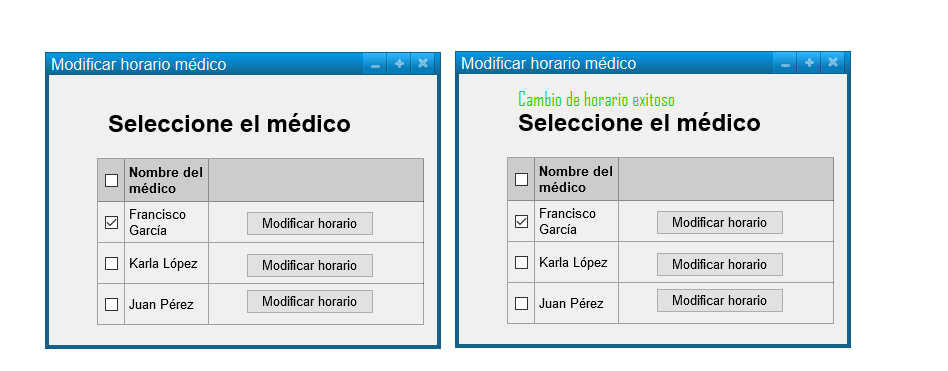
\includegraphics[width=1\textwidth]{images/UI5Gerente2}
    \caption{Listado de médicos}
\end{figure}

\subsubsection{Entradas}
  Ninguna

\subsubsection{Comandos}
\begin{itemize}
    \item \IUbutton{Modificar horario}: Permite modificar el horario del médico.
\end{itemize}

\subsubsection{Mensajes}
{\em MSG5a-}: ''Cambio de horario exitoso''.


   
\subsection{UI7 Pantalla horario de médicos}

\subsubsection{Objetivo}
   Seleccionar un rango de horario de disponibilidad para un médico y, opcionalmente, su horario de comida.

\subsubsection{Diseño}
    Esta pantalla aparece al oprimir \IUbutton{Modificar horario} de la \IUref{UI6}{Pantalla modificar horario listado de médicos}.

\begin{figure}[htbp!]
  \centering
    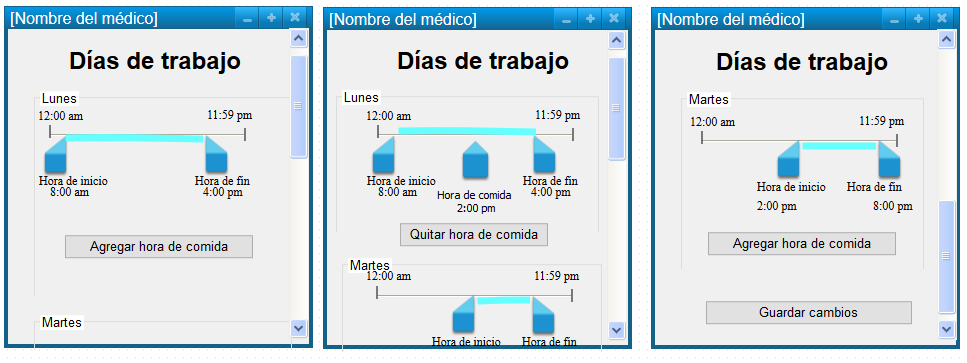
\includegraphics[width=1\textwidth]{images/UI5Gerente3}
    \caption{Listado de médicos}
\end{figure}

\subsubsection{Entradas}
\begin{itemize}
  \item Rango de horario de disponibilidad para consultas.
  \item Hora de comida para el médico (opcional).
\end{itemize}  
  

\subsubsection{Comandos}
\begin{itemize}
    \item \IUbutton{Agregar hora de comida}: Cambiar la selección de horario para agregar una hora de comida para el médico.
    \item \IUbutton{Quitar hora de comida}: Elimina el marcador de la hora de comida.
    \item \IUbutton{Guardar cambios}: Guarda los cambios realizados en el horario del médicos.
\end{itemize}

\subsubsection{Mensajes}
{\em MSG5b-}: ''La hora de comida debe de estar entre el rango de horario de disponibilidad.''.
 
 